\section{User Study}
To demonstrate our proposed method, we investigated whether the level of experienced presence impacts the spatial exploration behavior of participants in a beyond room-scale VR. Here, we used data from a study by Gehrke et al. that uses the \textit{invisible maze task} mimicking a real-world exploration situation such as finding your way in complete darkness~\cite{Gehrke2018, Miyakoshi2021-ni, Gehrke2021-ml}. We conducted the following two-step analysis. First, we constructed parametric maps to assess where participants exploration behavior was impacted as a function of experienced presence. To this end, we investigated fine-grained behavior at each single point in space by conducting mass-univariate pixel-by-pixel modeling of experienced presence on time spent at each location, i.e. pixel. To situate our findings on an individual differences level we followed up with a linear regression scheme, now using aggregated data. We predicted experienced presence using participants characteristics such as video game experience and perspective taking ability (see further details below).

\subsection{Participants, Procedure, Task and Setup} Thirty-two healthy participants (aged 21--45 years, 14 men) participated in the experiment~\cite{Gehrke2018, Gehrke2021-ml}. All participants gave written informed consent to participation and their experimental protocol was approved by the local ethics committee (protocol: GR\_08\_20170428). Three participants were excluded from data analysis due to incomplete data or difficulties in complying with task requirements.

\begin{figure}[!t]
\centering
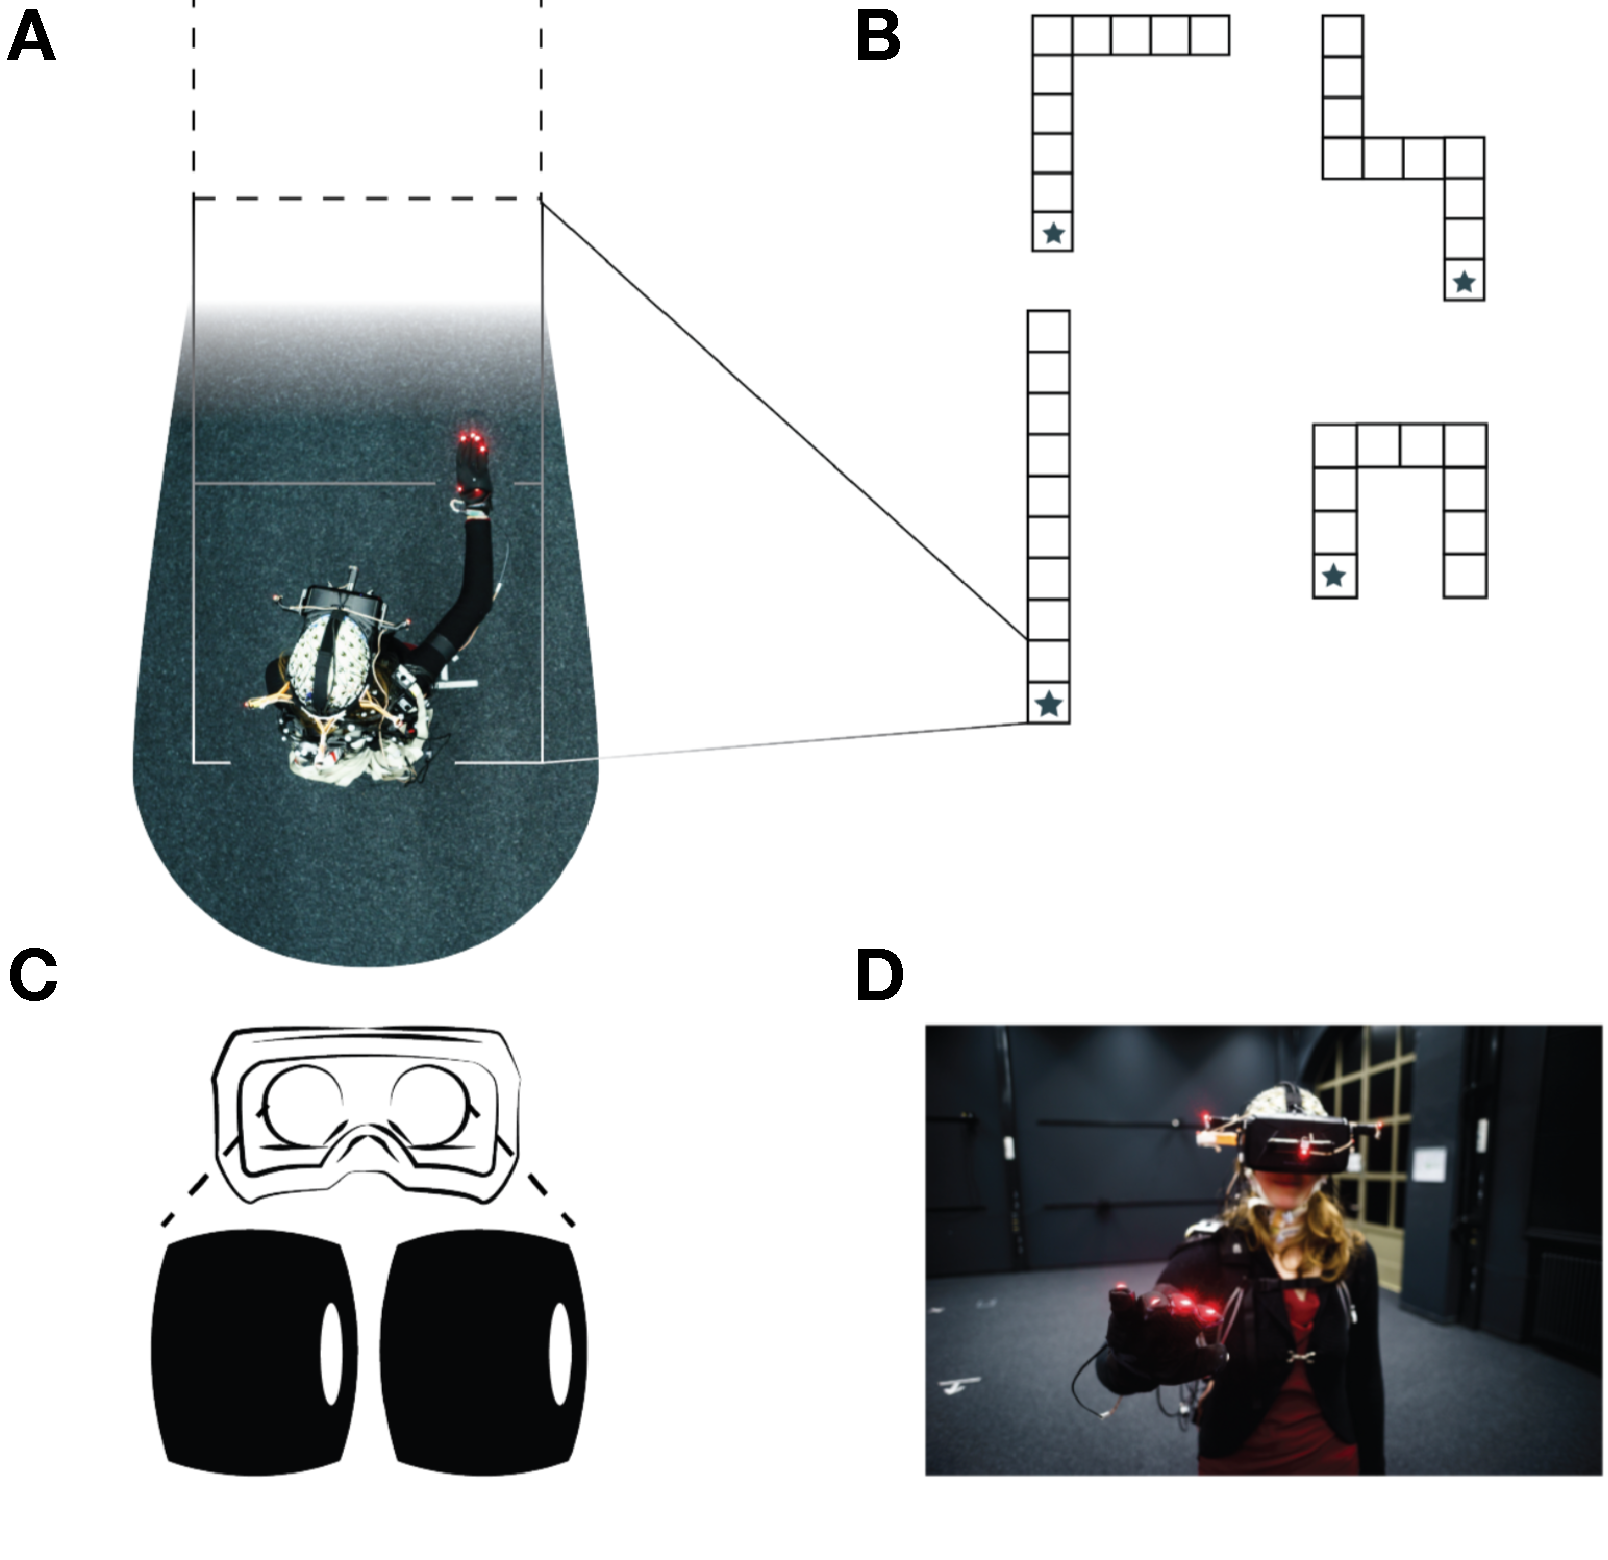
\includegraphics[width=\linewidth]{figures/IMT_Task.pdf}
\vspace{6pt}
\caption{Invisible Maze Task, \textbf{A,} Participant from a bird’s eye view. \textbf{B,} Participants were instructed to explore four different mazes and return to the start.~\cite{Gehrke2018}\textbf{C,} First-person view in binocular `VR optics' of a wall touch. \textbf{D,} Participants were equipped with 160 channels wireless EEG, head-mounted virtual reality goggles and LEDs for motion capture.}
% \Description{A: Top-down view of a participant exploring a virtual maze environment. B: Shapes of the different mazes, shapes are similar to letter I, L, Z and U. C: View inside of the VR headset show a sparse visual feedback occurring when participants touch a wall, much like navigating with a white cane. D: Portrait of a participant during a reach for a wall wearing an EEG Headset and a VR headset.}
\label{imt_task}
\end{figure}

\subsubsection{The Invisible Maze Task} In the experiment participants freely explore a sparse invisible maze environment by walking through virtual mazes and probing for visual feedback when touching the virtual wall of a 1m wide path with their \textit{right} hand. The stimuli were presented using an Oculus Rift DK2 VR headset in combination with a dedicated optical tracking system. Upon collision of the \textit{right} hand with an invisible wall, a white disc appears 30 cm behind the collision point parallel to the invisible wall much like the beam from a torch in a cave, see figure \ref{imt_task} C (consult~\cite{Gehrke2018} for extensive details on the task, instrumentation, and data collection). The left hand was not tracked and participants were instructed to keep the left arm close to their body. Performing the task, participants explored four different mazes in the order, `I', `L', `Z' and `U', see figure \ref{imt_task} B. The task was designed to emphasize participants internal build-up of a spatial representation of the maze layout. Doing the task, participants displayed a behavior that is reported to be comparable to explorative wall touches in the dark to find the way.

For each maze the procedure was as follows: participants were briefly disoriented and then positioned facing the open side of the path. Then, participants were directed to explore the invisible path until they reached a dead end, and subsequently to find their way back to the starting position. At the end of each maze trial, participants received a gamified feedback and were then asked to draw a sketch map of the maze from a bird’s eye view as an index of spatial learning. The procedure was repeated three times in a row for each maze to foster spatial learning. 

The complete experiment, including preparation of physiological measures (Electroencephalogram, EEG) took approximately 4 hours. Preceding and following the task, participants completed a set of questionnaires to assess demographics, spatial abilities, and presence. Synchronized motion capture was collected with behavioral events alongside high-density EEG. For the inquiry in this paper, data of the three exploration phases were aggregated.

\subsubsection{Assessing presence} To assess experienced presence, the igroup presence questionnaire~\cite{Schubert2003} was administered following each individual maze exploration. For our analyses only the first item of the questionnaire was considered, the general subjective presence measure (G1), which represents the sense of being in a place, i.e. `In the computer generated world I had a sense of "being there"' rated from `not at all' to `very much' on a 7-point Likert scale~\cite{Schubert2003, Slater1993}.

%%%%%
%We considered a data-driven approach to finding a useful, i.e. scalable, classification model. Therefore, we initially included a variety of participant descriptors which were subsequently reduced to a set with highest explanatory power. In this way, we progressed towards a minimal model allowing other researchers to reproduce our findings.